\section{Peierls' argument}
\label{sec:peierls}

\begin{figure}[b]
    \includegraphics{figures/triangular.pdf}
    \caption{The triangular lattice graph $\T_3$ with $+$ spins on the boundary.}
    \label{fig:triangular}
\end{figure}

Peierls disproved Ising's conjecture for the absence of phase transition
in dimension $d\geq 2$.
For simplicity, we state and prove his result on the two-dimensional triangular lattice graph.
The triangular lattice $\T$ is the nearest-neighbour graph on the vertex set $\Z+\Z e^{i\pi/3}\subset\C$.
We write $\T_n$ for the subgraph induced by vertices at a graph distance of at most $n$ from the origin,
and $\partial\T_n$ for the set of vertices at a graph distance of exactly $n$ from the origin.
We are interested in the Ising model on $\T_n$ with $+$ boundary conditions imposed on $\partial\T_n$,
see Figure~\ref{fig:triangular}.

\begin{theorem}[Peierls, 1936]
    \label{thm:peierls}
    For sufficiently large $\beta\in[0,\infty)$, we have
    \[
        \inf_n\mu_{\T_n,\beta}[\sigma_0|\{\sigma|_{\partial\T_n}\equiv +\}]>0.
    \]
    In other words, the centre spin remains positively correlated with the boundary,
    uniformly in the system size.
\end{theorem}

Before proving this theorem, we consider the combinatorics of the Ising model on the triangular lattice.
Consider any spin configuration $\sigma$ on $\T_n$ with $+$ boundary conditions.
Figure~\ref{fig:peierls} (Left) depicts such a configuration.
In the figure, we represented the vertices by hexagons in such a way that they fill up the space.
Although this is no more than a visual trick, the picture suggests that $\sigma$ can be represented by a collection of \emph{loops}.

We now make this formal.
Let $\T_n^*=(V_n^*,E_n^*)$ denote the \emph{dual graph} of $\T_n$.
Its vertex set is the set of centres of triangles of $\T_n$.
Its edge set connects nearest-neighbour vertices.
See Figure~\ref{fig:peierls} (Right).
For any spin configuration $\sigma$ on $\T_n$ which equals $+$ on $\partial\T_n$,
we define its \emph{interface} $\calI(\sigma)\subset E_n^*$ as the set of dual edges separating two spins with a distinct value.
See Figure~\ref{fig:peierls} for such a spin configuration $\sigma$ and its interface $\calI(\sigma)$.

\begin{figure}[b]
    \includegraphics{figures/Peierls.pdf}
    \caption{
        Left: A spin configuration $\sigma$ on $\T_3$ with $+$ boundary conditions.
        The spins are represented by hexagons in such a way that they fill up the space.
        Right: The triangular lattice graph $\T_3$ (in grey)
        and its planar dual $\T_3^*$ (in black).
        It also depicts the loops of the interface $\calI(\sigma)$ for the configuration $\sigma$ on the left.
    }
    \label{fig:peierls}
\end{figure}

\begin{definition}[Loop configuration]
    A \emph{loop configuration} on $\T_n$ is a subset $\gamma\subset E_n^*$ giving
    an even degree to every vertex of $V_n^*$.
\end{definition}

\begin{lemma}[Loop representation of the Ising model on the triangular lattice]
    \label{lem:peierls_loop_representation}
    Fix $n$ and $\beta$.
    All of the following are true.
    \begin{enumerate}
        \item The map $\sigma\mapsto\calI(\sigma)$ is a bijection from the set of spin configurations $\sigma$ on $\T_n$
        with $\sigma|_{\partial\T_n}\equiv +$ to the set of loop configurations on $\T_n$.
        \item If $\sigma$ is such a spin configuration, then
        \begin{equation}
            \label{eq:peierls_reconstruction}
            \sigma_u = (-1)^{\text{the number of loops of $\calI(\sigma)$ surrounding $u$}}.
        \end{equation}
        \item For any loop configuration $\gamma$, we have
    \begin{equation}
        \label{eq:peierls_energy}
        \mu_{\T_n,\beta}[\{\calI(\sigma)=\gamma\}]\propto e^{-2\beta|\gamma|}.
    \end{equation}
    \end{enumerate}
\end{lemma}

\begin{proof}
    \begin{itemize}
        \item\textbf{Proof that $\calI(\sigma)$ is a loop configuration.} It is easy to see from Figure~\ref{fig:peierls} that $\calI(\sigma)$
        is a loop configuration for any spin configuration $\sigma$ on $\T_n$
        that equals $+$ on $\partial\T_n$.
        \item\textbf{Proof that $\calI$ is a bijection and Equation~\eqref{eq:peierls_reconstruction} holds.}
        Now consider any loop configuration $\gamma$.
        Define the spin configuration $\sigma$ by
        \[
            \sigma_u = (-1)^{\text{the number of loops of $\gamma$ surrounding $u$}}.
        \]
        Then it is easy to see that $\sigma|_{\partial\T_n}\equiv +$,
        and that $\calI(\sigma)=\gamma$.
        This proves that $\calI$ is a bijection, and that Equation~\eqref{eq:peierls_reconstruction} holds.
        \item\textbf{Proof of Equation~\eqref{eq:peierls_energy}.}
        Notice that $|\calI(\sigma)|$ equals the number of $\T_n$-edges
        on which $\sigma$ disagrees.
        In particular, we have
        \[
            H(\sigma)=-\beta\sum_{u\sim v}\sigma_u\sigma_v=
            -\beta\sum_{u\sim v}1 + 2\beta|\calI(\sigma)|,
        \]
        from which it follows that
        \[
            \mu_{\T_n,\beta}[\{\calI(\sigma)=\gamma\}]\propto
            e^{-2\beta|\gamma|}.
        \]
    \end{itemize}
    We have now proved the desired statements.
\end{proof}

\begin{lemma}[The energy of a loop]
    Fix $n$ and $\beta$.
    Then for any loop configuration $\gamma$, we have
    \[
        \mu_{\T_n,\beta}[\{\gamma\subset\calI(\sigma)\}]\leq e^{-2\beta|\gamma|}.
    \]
\end{lemma}

\begin{proof}
    It suffices to prove that
    \[
        \frac{
            \mu_{\T_n,\beta}[\{\gamma\subset\calI(\sigma)\}]
        }
        {
            \mu_{\T_n,\beta}[\{\gamma\cap\calI(\sigma)=\emptyset\}]
        }
        = e^{-2\beta|\gamma|}.
    \]
    Let $L$ denote the set of loop configurations $\gamma'$ which are disjoint from $\gamma$.
    Then the left hand side of the above equation equals
    \[
        \frac{
            \sum_{\gamma'\in L} e^{-2\beta|\gamma'\cup\gamma|}
        }
        {
            \sum_{\gamma'\in L} e^{-2\beta|\gamma'|}
        }
        =
        \frac{
            \sum_{\gamma'\in L} e^{-2\beta|\gamma'|}e^{-2\beta|\gamma|}
        }
        {
            \sum_{\gamma'\in L} e^{-2\beta|\gamma'|}
        }
        =
        e^{-2\beta|\gamma|}.
    \]
    This implies the desired bound.
\end{proof}

By a \emph{loop}, we simply mean a connected component of a loop configuration.

\begin{lemma}[The entropy vs.\ energy calculation]
    Fix $n$ and $\beta$,
    and consider a dual edge $uv\in E_n^*$.
    Then for any $\ell\in\Z_{\geq 1}$,
    \[
        \mu_{\T_n,\beta}[\{\text{$uv$ belongs to a $\calI(\sigma)$-loop of length $\ell$}\}]
        \leq (2e^{-2\beta})^\ell.
    \]
    In particular, if $2e^{-2\beta}<1$, then 
    \[
        \mu_{\T_n,\beta}[\{\text{$uv$ belongs to a $\calI(\sigma)$-loop of length $\geq\ell$}\}]
        \leq \frac{(2e^{-2\beta})^\ell}{1-2e^{-2\beta}}.
    \]
\end{lemma}

\begin{proof}
    Let $L$ denote the set of loops of length $\ell$ through $uv$.
    Notice that $|L|\leq 2^\ell$.
    Then
    \begin{multline}
        \mu_{\T_n,\beta}[\{\text{$uv$ belongs to a $\calI(\sigma)$-loop of length $\ell$}\}]
        \\=
        \sum_{\gamma\in L} \mu_{\T_n,\beta}[\{\gamma\subset\calI(\sigma)\}]
        \leq
        \sum_{\gamma\in L} e^{-2\beta|\gamma|}
        \leq
         (2e^{-2\beta})^\ell.
    \end{multline}
    This is the desired bound.
    The second bound follows by working out the geometric series.
\end{proof}

The second bound tells us that if $2e^{-2\beta}<1$,
then the energy cost of a long loop is so high that the length of a loop
through a given edges has an exponential tail.
This is the key to proving Theorem~\ref{thm:peierls}.

\begin{proof}[Proof of Theorem~\ref{thm:peierls}]
    It suffices to prove that
    \[
        \mu_{\T_n,\beta}[\{\sigma_0=-\}|\{\sigma|_{\partial\T_n}\equiv +\}]
        \leq \frac13.
    \]
    By the loop representation (Lemma~\ref{lem:peierls_loop_representation}),
    if $\sigma_0=-$, then $\calI(\sigma)$ contains at least one loop around $0$.
    Therefore it suffices to prove that
    \[
        \mu_{\T_n,\beta}[\{\text{$\calI(\sigma)$ contains a loop around $0$}\}]
        \leq \frac13.
    \]
    Any such loop must hit the half-line starting at $0$ and going straight up
    (the blue line in Figure~\ref{fig:peierls}, Right).
    Enumerate the horizontal edges of $E_n^*$ intersecting this half-line by $(e_i)_{i\geq 1}$.
    Thus, if $\calI(\sigma)$ contains a loop around $0$, then it must contain a loop of length at least $i$ through $e_i$ for some $i\geq 1$.
    In particular, we get
    \begin{multline}
        \mu_{\T_n,\beta}[\{\sigma_0=-\}|\{\sigma|_{\partial\T_n}\equiv +\}]
        \\\leq
        \sum_{i=1}^\infty \mu_{\T_n,\beta}[\{\text{$\calI(\sigma)$ contains a loop of length at least $i$ through $e_i$}\}]
        \\\leq
        \sum_{i=1}^\infty \frac{(2e^{-2\beta})^i}{1-2e^{-2\beta}}
        =
        \frac{2e^{-2\beta}}{(1-2e^{-2\beta})^2}.
    \end{multline}
    The bound on the right is uniform in $n$,
    and tends to zero as $\beta$ tends to infinity.
\end{proof}

\begin{exercise}[Peierls argument on the square lattice]
    Fix $d=2$.
    Now let $G_n$ be the nearest-neighbour graph on the vertex set $\Z^d\cap [-n,n]^d$.
    Write $\partial G_n$ for the vertices of $G_n$ at an $\ell^\infty$-distance of exactly $n$ from the origin.
    Prove that for sufficiently large $\beta$, we have
    \[
        \inf_n\mu_{G_n,\beta}[\sigma_0|\{\sigma|_{\partial G_n}\equiv +\}]>0.
    \]
    \emph{Hint.}
    The natural analogue of ``loop configurations'' are
    ``interface configurations'', which are subsets $\gamma$ of the dual edges
    such that every dual vertex is given an even degree by $\gamma$.
    It is now possible that $\gamma$ gives degree four to some dual vertices.
    While this means that the connected components of $\gamma$ are not necessarily loops,
    it is still possible to implement the argument above with minimal modifications.
\end{exercise}

\begin{exercise}[Harder: Peierls argument in higher dimensions]
    Prove the same results in any fixed dimension $d\in\Z_{>2}$.
\end{exercise}



% The even degree requirement on $\gamma$ is very restrictive.
% Since the max-degree of $\T_n^*$ is three,
% every vertex of $(V_n^*,\gamma)$ has degree zero or two.
% Therefore $\gamma$ is a disjoint union of self-avoiding finite loops.







% \begin{proof}
%     Our objective is to prove that $\P_{\Lambda_n,\beta}^+[\{\sigma_{(0,0)}=-\}]\leq\frac13$
%     for all $n$.
%     Fix $n$.

%     Consider the set $\Omega'\subset\Omega$ of spin configurations on $\bar\Lambda_n$
%     which assign $+$ to $\partial\Lambda_n$.
%     The two-dimensional square lattice graph $G=\Z^2$ is planar, and
%     therefore we may consider its planar dual $G^*$.
%     For any spin configuration $\sigma\in\Omega'$,
%     we let $\calI(\sigma)\subset E(G^*)$ denote its \emph{interface},
%     that is, the set of dual edges separating two spins with a \emph{distinct} value.
%     Notice that:
%     \begin{itemize}
%         \item The map $\sigma\mapsto \calI(\sigma)$ is injective,
%         \item If $\sigma_{(0,0)}=-$, then $\calI(\sigma)$ contains at least one self-avoiding loop around $(0,0)$.
%     \end{itemize}
%     In particular, inclusion of events yields
%     \begin{equation}
%         \label{eq:peierlsgeneral}
%         \P_{\Lambda_n,\beta}^+[\{\sigma_{(0,0)}=-\}]
%         \leq
%         \P_{\Lambda_n,\beta}^+[\{\text{$\calI(\sigma)$ contains a loop $\gamma$ around $(0,0)$}\}].
%     \end{equation}

%     We would now like to make a competition between entropy and energy appear,
%     as for the Curie-Weiss model.
%     The entropy comes from the choice of the loop $\gamma$;
%     the energy comes into play when upper bounding the probability that a particular loop
%     belongs to $\calI(\sigma)$.
%     For large $\beta$, energy wins over entropy, yielding the desired bound.
%     Let us start with the energy bound.

%     \begin{claim*}
%         For any fixed loop $\gamma$, we may bound $\P_{\Lambda_n,\beta}^+[\{\gamma\subset\calI(\sigma)\}]\leq e^{-2\beta|\gamma|}$.
%     \end{claim*}

%     \begin{proof}[Proof of the claim]
%     We would like to define a \emph{loop erasure map} $\calE:\{\gamma\subset\calI(\sigma)\}\to\Omega'$,
%     which has the property that it removes the loop $\gamma$ from the interface,
%     that is,
%     \[
%         \calI(\calE(\sigma))=\calE(\sigma)\setminus\gamma.
%     \]
%     It is easy to realise such a map: we simply define $\calE$ such that it
%     flips the sign of every vertex of $\Lambda_n$ which is surrounded by $\gamma$.
%     Since $\calI$ is injective, the map $\calE$ is also injective,
%     and we have
%     \[
%         \P_{\Lambda_n,\beta}^+[\{\gamma\subset\calI(\sigma)\}]
%         =
%         \frac
%         {\sum_{\sigma\in\operatorname{Domain}(\calE)}e^{-H(\sigma)}}
%         {\sum_{\sigma\in\Omega'}e^{-H(\sigma)}}
%         \leq
%         \frac
%         {\sum_{\sigma\in\operatorname{Domain}(\calE)}e^{-H(\sigma)}}
%         {\sum_{\sigma\in\operatorname{Image}(\calE)}e^{-H(\sigma)}}
%         =
%         e^{-2\beta|\gamma|}.
%     \]
%     The last equality is easy,
%     since for any $\sigma\in\{\gamma\subset\calI(\sigma)\}$,
%     we have
%     \[
%         H(\calE(\sigma))=H(\sigma)-2\beta|\gamma|,
%     \]
%     since $\calE$ removes precisely $|\gamma|$ disagreement edges from the interface.
%     This proves the claim.
%     \renewcommand{\qedsymbol}{}
%     \end{proof}

%     We use the energy bound to prove another interesting intermediate result.

%     \begin{claim*}[Exponential decay of the loop length]
%         For any dual edge $e$, we have
%         \[
%         \P_{\Lambda_n,\beta}^+[\{\text{$\calI(\sigma)$ contains a loop of length at least $\ell$ through $e$}\}]
%         \leq (3e^{-2\beta})^\ell \frac{1}{1-3e^{-2\beta}}
%         \]
%         whenever $3e^{-2\beta}<1$.
%     \end{claim*}

%     \begin{proof}[Proof of the claim]
%         Let $\calL_k$ denote the set of self-avoiding loops through $e$
%         of length $k$.
%         Notice that $|\calL_k|\leq 3^k$.
%         A union bound yields
%         \begin{multline}
%             \P_{\Lambda_n,\beta}^+[\{\text{$\calI(\sigma)$ contains a loop of length at least $\ell$ through $e$}\}]
%             \\
%             \leq
%             \sum_{k=\ell}^\infty \sum_{\gamma\in\calL_k} 
%             \P_{\Lambda_n,\beta}^+[\{\gamma\subset\calI(\sigma)\}]
%             \leq
%             \sum_{k=\ell}^\infty |\calL_k|\cdot e^{-2\beta k}
%             \leq 
%             \sum_{k=\ell}^\infty 3^k\cdot e^{-2\beta k}
%             \\
%             =
%             (3e^{-2\beta})^\ell \frac{1}{1-3e^{-2\beta}}.
%         \end{multline}
%         This is the desired bound.
%     \renewcommand{\qedsymbol}{}
%     \end{proof}

%     Return to Equation~\eqref{eq:peierlsgeneral}.
%     If $\calI(\sigma)$ contains a loop around $(0,0)$, then this loop 
%     must hit $(k-\frac12,0)$ for some $k\in\Z_{\geq 1}$,
%     and this loop must have at least $k$ steps.
%     Thus, another union bound yields
%     \[
%         \P_{\Lambda_n,\beta}^+[\{\sigma_{(0,0)}=-\}]
%         \leq
%         \sum_{k=1}^\infty 
%         (3e^{-2\beta})^{k} \frac{1}{1-3e^{-2\beta}}
%         =(3e^{-2\beta})\frac{1}{(1-3e^{-2\beta})^2}.
%     \]
%     The right hand side is smaller than $\frac13$ when $\beta$ is sufficiently large,
%     independently of $n$.
% \end{proof}

% \begin{remark*}
%     Peierls' is robust,
%     in the sense that it can be adapted to many other models in statistical mechanics.
% \end{remark*}

% \begin{exercise}[The Peierls argument in higher dimensions]
%     \label{exo:peierls_general}
%     Now consider the square lattice graph $\Z^d$ in dimension $d\geq 3$.
%     What is the structure of the interface in this case?
%     Can we adapt Peierls' to prove magnetisation for sufficiently large $\beta$?
% \end{exercise}
